Das Frontend, genauer gesagt das Profilmanagement, wurde in Angular entwickelt. Die einzelnen Seiten sind eigene Komponenten. Die Navigationsleiste ist die einzige Komponente, welche dauerhaft in der Webanwendung zu sehen ist.

\begin{lstlisting}[language=html, caption=Navigationsleiste Komponente]
    <div class="content">
  <div class="leftSide">
    <div class="logo">
      <h1>APERTA</h1>
    </div>
  </div>
  <div class="pageList">
    <div class="page"><a href="keyPadSettings">Key Pad</a></div>
    <div class="page"><a href="signSettings">Sign</a></div>
    <div class="page"><a href="nfcSettings">NFC</a></div>
    <div class="page"><a href="profile"><img src="../../../assets/profil.png"> </a></div>
    <div class="page"><a href="login">Login</a></div>
  </div>
</div>
\end{lstlisting}

In den Div-Containern „pageList“ befinden sich die Verlinkungen auf die einzelnen Komponenten. Mittels <a> Tag werden die Links zu den Komponenten angegeben. Diese werden dann durch das im app.module.ts angegeben Routing in die View geladen.

\subsubsection{DIV Container}

DIV ist eine Abkürzung für den Begriff „division“ (=Bereich). Sie dienen zur Gestaltung der Website. Ein DIV-Container ist im Grunde genommen ein leerer Rahmen und begrenzt einen Bereich. 
\cite{DivContainer}

\subsubsection{<a>-Tag}
Der Anchor Tag ist einer der vielen HTML-Tags. Er definiert den Anfangs- und Endpunkt eines Hyperlinks, welcher eine Website oder die Unterseiten in einem Projekt miteinander verlinkt.
\cite{ATag}

\begin{lstlisting}[language=html, caption=Profil Komponente]
    <div class="container">
  <div class="divMainContent">
    <div class="divLeftContent">
      <h1>My Profile</h1>
      <h2>Settings</h2>

      <div class="Form">
        <form class="formProfileSettings" name="formProfileSettings">
          <div class="divNameSettings">
            <div class="Firstname">
              <label name="lbFirstName">First Name</label>
              <input name="txFirstName" type="text" placeholder="First Name">
            </div>
            <div class="Lastname">
              <label name="lbLastName">Last Name</label>
              <input name="txLastName" type="text" placeholder="Last Name">
            </div>
          </div>
          <div class="divPersonalSettings">
            <div class="Birthday">
              <label name="lbBirthday">Birthday</label>
              <input name="dtBirthday" type="date">
            </div>
            <div class="Phonenumber">
              <label name="lbPhonenumber">Phonenumber</label>
              <input name="nbPhonennumber" type="tel" placeholder="+43 660 123 123 12">
            </div>
          </div>
          <div class="divPersonalSettings">
            <div class="City">
              <label name="lbCity">City</label>
              <input name="txCity" type="text" placeholder="Linz">
            </div>
            <div class="Postcode">
              <label name="lbPostcode">Postcode</label>
              <input name="nbPostcode" type="number" placeholder="4020">
            </div>
          </div>


          <div class="divButton">
            <button class="btSubscribe" name="btSubscribe">Save</button>
          </div>
        </form>
        <hr class="horizontalLine">
      </div>
      <div class="divMoreSettings">
        <a href="/keyPadSettings">Key-Pad Settings</a>
        <a href="#">NFC Settings</a>
        <a href="/signSettings">Sign Settings</a>
      </div>
    </div>
    <div class="verticalLine"></div>
    <div class="divRightContent">
      <div class="ActiveSignh2"><h2>Active Sign</h2></div>
      <div class="divActiveSigns">
        <app-sign *ngFor="let a of fakeArray; let index = index" [licensename]="licensename"></app-sign>

      </div>
        <div class="divButton">
          <button class="btSubscribe" name="AddMore"><a href="/addSign">Add More</a></button>
        </div>

      <hr class="horizontalLineRight">
      <div class="Moreh2">
        <h2>More</h2>
        <div class="divButton">
          <button class="btSubscribe" name="AddMore">Add More</button>
        </div>
      </div>
      <div class="divMore">
        <div class="Components">
          <div class="ComponentsName">Key-Pad</div>
          <div class="ComponentPic">
            <img src="../../../assets/keypad.png" alt ="Key Pad"/>
          </div>
          <div class="MoreCheckbox">
            <div class="CheckActive">
              <img src="../../../assets/checkmark-outline.svg" alt="Checkmark" />
            </div>
            <div class="CheckInactive">
              <img src="../../../assets/close-outline.svg" />
            </div>
          </div>
        </div>
        <div class="Components">
          <div class="ComponentsName">NFC-Chip</div>
          <div class="ComponentPic">
            <img src="../../../assets/nfc.png" alt ="NFC-Chip"/>
          </div>
          <div class="MoreCheckbox">
            <div class="CheckActive">
              <img src="../../../assets/checkmark-outline.svg" alt="Checkmark" />
            </div>
            <div class="CheckInactive">
              <img src="../../assets//close-outline.svg" />
            </div>
          </div>
        </div>
      </div>
    </div>
  </div>
</div>
\end{lstlisting}

In der Profil-Komponente werden die Bauteile, die im Besitz des Users oder der Userin sind, angezeigt. Darüber können im Profil die Entscheidungen getroffen werden. Die Komponenten werden in den Tags <app-sign>, <app-keypad> und <app-nfc> geladen und dargestellt. Über die <input>-Tags kann der Benutzer oder die Benutzerin das Konto mit persönlichen Informationen erweitern. Die Input Felder befinden sich in einem <form>-Tag. Die DIV-Boxen „Checkactive“ und „CheckInactive“ dienen dazu, ob ein Bauteil zurzeit aktiviert oder deaktiviert ist.

\subsubsection{<form>}
Der form-Tag beinhaltet die Felder des Formulars und ist für die Verarbeitung der Eingaben der Nutzerin oder des Nutzer, mittels action und method zuständig.
\cite{Form}

\subsubsection{<input>}
Der Tag wird genutzt, um ein Eingabeelement zu definieren. Er ermöglich der Nutzerin oder dem Nutzer die Eingabe von Daten.
\cite{InputTag}

\subsubsection{<Komponenten Tag>}
Um eine Komponente von Angular einzubinden, wird der Komponenten Tag verwendet. 

\subsubsection{*ngFor}
Eine For-Schleife wird verwendet, um den Code mehrmals zu durchzulaufen oder um Daten anzuzeigen. Beim ngfor wird ein Array, Element für Element durchlaufen und gibt sie als HTML-Syntax aus. Die for-Schleife wird in das Element geschrieben, welches mehrmals wiederholt werden soll. Im Falle der Profil-Seite wird es genutzt, um mehrere Kennzeichen auszugeben. Es werden immer die 3 aktuellsten Kennzeichen ausgegeben.
\cite{NgFor}

\subsubsection{Binding}
Es gibt verschiedene Wege für das Binding in Angular. Sie erlauben die Kommunikation zwischen HTML und TypeScript. In der Profil-Komponente wurde das Property Binding verwendet. Durch das Property Binding wird eine Variable mit einer DOM-Property, HTML Attributen, Direktive oder Komponente Properties verbunden. Die Kommunikationsrichtung dabei ist von TypeScript-Datei zu HTML-Datei.
\cite{Binding}
\pagebreak
\begin{lstlisting}[caption=KeyPad Model]
    export class KeyPad {
  Id : number = 0;
  numpad_id : number = 0;
  numpad_code : String = "";
  active: boolean = false;
}
\end{lstlisting}

Das KeyPad Model ist ein Beispiel für alle Models in unserem Projekt. In einer Modelklasse befinden sich alle Variablen, die auch in der Datenbank vorhanden sind. Somit kann ein Datenbankeintrag ganz einfach in eine Komponente gebracht und verarbeitet werden. 

\begin{lstlisting}[language=HTML, caption=Login Komponente]
    <section class="user">
    <div class="user_options-container">
      <div class="user_options-text">
        <div class="user_options-unregistered">
          <h2 class="user_unregistered-title">Don't have an account yet?</h2>
          <button class="user_unregistered-signup" id="signup-button">Sign up</button>
        </div>
  
        <div class="user_options-registered">
          <h2 class="user_registered-title">Already have an account?</h2>
          <button class="user_registered-login" id="login-button">Login</button>
        </div>
      </div>
  
      <div class="user_options-forms" id="user_options-forms">
        <div class="user_forms-login">
          <h2 class="forms_title">Login</h2>
          <form class="forms_form">
            <fieldset class="forms_fieldset">
              <div class="forms_field">
                <input type="email" placeholder="Email" class="forms_field-input" required autofocus />
              </div>
              <div class="forms_field">
                <input type="password" placeholder="Password" class="forms_field-input" required />
              </div>
            </fieldset>
            <div class="forms_buttons">
              <button type="button" class="forms_buttons-forgot">Forgot password?</button>
              <input type="submit" value="Log In" class="forms_buttons-action">
            </div>
          </form>
        </div>
        <div class="user_forms-signup">
          <h2 class="forms_title">Sign Up</h2>
          <form class="forms_form">
            <fieldset class="forms_fieldset">
              <div class="forms_field">
                <input type="text" placeholder="Full Name" class="forms_field-input" required />
              </div>
              <div class="forms_field">
                <input type="email" placeholder="Email" class="forms_field-input" required />
              </div>
              <div class="forms_field">
                <input type="password" placeholder="Password" class="forms_field-input" required />
              </div>
            </fieldset>
            <div class="forms_buttons">
              <input type="submit" value="Sign up" class="forms_buttons-action">
            </div>
          </form>
        </div>
      </div>
    </div>
  </section>  
\end{lstlisting}

Die Login-Komponente stellt in unserem Projekt die Seite dar, auf der sich angemeldet oder registriert werden kann. Sie verwendet einfache Input Felder für die Eingabe der Daten. Diese werden dann an die Datenbank weitergeleitet und verarbeitet.

\subsubsection{<section>}
Der section-Tag stellt eine Unterteilung des Dokuments dar. Etwa eine thematische Gruppierung des Inhaltes, typischerweise mit einer Überschrift. Die section sollte identifizierbar sein.
\cite{SectionTag}


\begin{figure}[h]
  \centering
  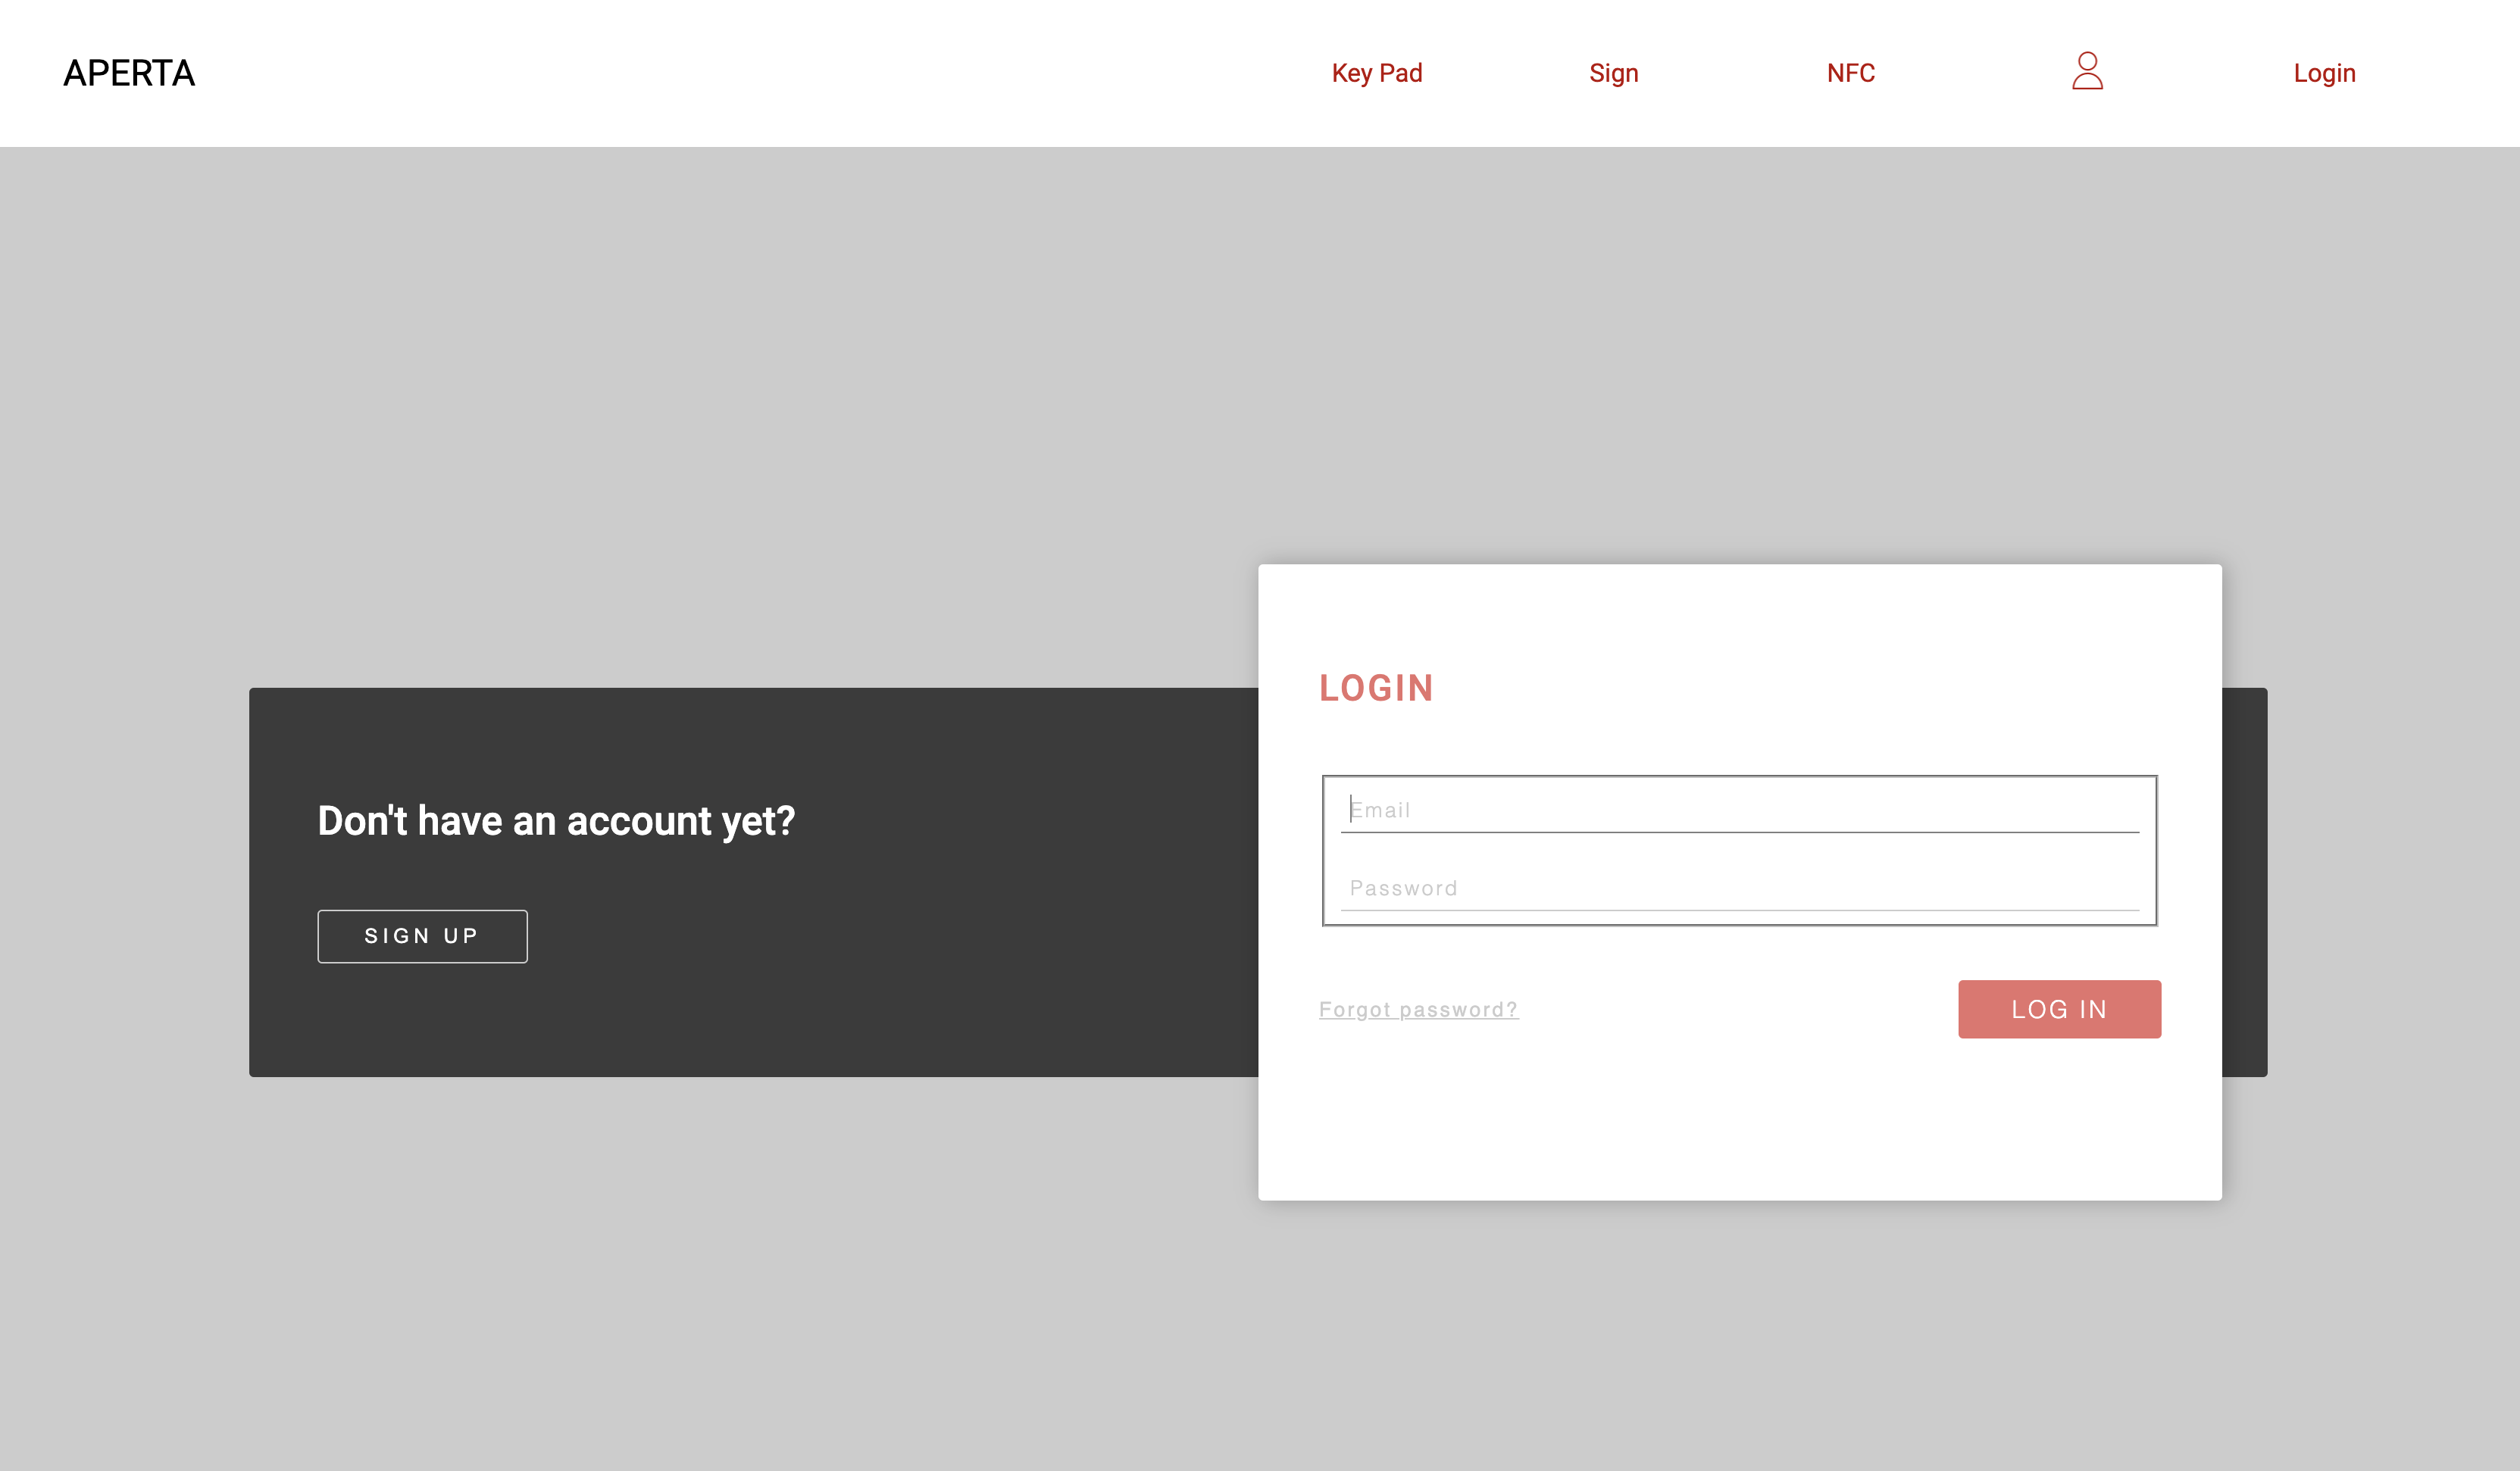
\includegraphics[width=0.8\textwidth]{pics/Loginseite.png}
  \caption{Loginseite}
\end{figure}
\pagebreak

\begin{lstlisting}[language=typeScript, caption=profile.component.ts]
    import { Input } from '@angular/core';
    import { Component, OnInit } from '@angular/core';
    import { Sign } from 'src/app/Model/sign';
    
    import {HttpService} from "../../Service/http.service";
    import { SignComponent } from '../sign/sign.component';
    
    @Component({
      selector: 'app-profile',
      templateUrl: './profile.component.html',
      styleUrls: ['./profile.component.css']
    })
    export class ProfileComponent implements OnInit {
    
      Signs: Sign[] | undefined;
      licensename : String = "";
      i: number = 0;
    
      constructor(private httpService: HttpService) { }
    
      ngOnInit(): void {
        this.getSigns();
      }
    
      fakeArray = new Array(3);
    
    
      getSigns(){
        this.httpService.getSigns().subscribe((data:Sign[])=>{
          this.Signs = data;
          console.log(data);
          this.getSignName();
        })
      }
    
      getSignName() {
        while (this.i <= 2) {
          this.licensename = this.Signs![this.i].licenseplate;
          console.log(this.licensename); 
          this.i++;
    
        }
      }
    
    }    
\end{lstlisting}

Die Profil-Komponente verarbeitet die Daten für die Kennzeichen. Mit der Funktion getSigns() werden die Daten vom http-service verarbeitet. Es werden die gesamten Daten in einem Array von Kennzeichen gespeichert. Mit der Methode getSignName() wird der Array, mithilfe einer while-Schleife durchlaufen, dabei werden die Strings der Kennzeichen auf eine Variable gespeichert. Diese werden dann, in der Webapplikation dargestellt.

\subsubsection{HttpService}
Mit this.httpService kann auf die Service Klasse zugegriffen werden. Diese stellt die gängigsten HTTP-Methoden zur Verfügung. Somit kann in der Komponente auf die Funktion getSigns(), welche im http-Service definiert ist, zugegriffen und ihre Werte verarbeitet werden.
\cite{HttpService}

\begin{lstlisting}[language=typeScript, caption=http.service.ts]
    import { Injectable } from '@angular/core';
import { HttpClient} from "@angular/common/http";
import {Sign} from "../Model/sign";
import { KeyPad } from '../Model/key-pad';
import { Nfc } from '../Model/nfc';



@Injectable({
  providedIn: 'root'
})
export class HttpService {
  baseUrl = "http://130.162.215.116";

  constructor(private http: HttpClient) { }

  getSigns(){
    var licenseplate = this.http.get<Sign[]>(this.baseUrl + "/get-licenseplates")
    return licenseplate
  }

  getKeyPads(){
    var keyPad = this.http.get<[]>(this.baseUrl + "/get-numpad-codes")
    return keyPad;
  }

  getNFC(){
    var nfc = this.http.get<[]>(this.baseUrl + "/get-rfid-codes")
    return nfc;
  }

  createNumpad(keypad: KeyPad){
    return this.http.post<KeyPad>(this.baseUrl + "/add-numpad", keypad)
  }

  createLicenseplate(licenseplate: Sign){
    return this.http.post<KeyPad>(this.baseUrl + "/add-licenseplate", licenseplate)
  }

  createRfid(rfid: Nfc){
    return this.http.post<KeyPad>(this.baseUrl + "/add-rfid", rfid)
  }

  deleteNumpad(numpad: KeyPad){
    return this.http.delete<KeyPad>(this.baseUrl + "/delete-numpad")
  }

  deleteLicenseplate(licenseplate: Sign){
    return this.http.delete<KeyPad>(this.baseUrl + "/delete-licenseplate")
  }

  deleteRfid(nfc: Nfc){
    return this.http.delete<KeyPad>(this.baseUrl + "/delete-rfid")
  }
}
\end{lstlisting}

Die baseUrl ist die Referenz zur Datenbank. Über diesen Link ist die Datenbank erreichbar. Mit den richtigen Endungen stellt sie einige Funktionen zur Verarbeitung der Einträge in der Datenbank zur Verfügung.

Die Funktionen getSigns(), getKeyPads() und getNFC() sind dazu da, um die Datenbankeinträge zu laden. Die Einträge der Datenbank kommen im return-Wert als JSON-Array zurück. Danach können sie in den Komponenten weiterverarbeitet werden.
Die Funktionen createNumpad(), createLicensplate() und createRfid() erzeugen einen neuen Eintrag in der Datenbank. Sie bekommen jeweils ein Element mitgegeben, das die Variablen aus der Datenbank belegt hat. Die Variablen werden von den Komponenten erzeugt.
deleteNumpad(), deleteLicenseplate() und deleteRfid() löschen jeweils den gewünschten Eintrag. Dazu bekommen sie das zu löschende Element als Parameter übergeben.


\subsubsection{HttpClient}
Unsere Front-End-Anwendung kommuniziert, so wie die meisten, über das HTTP-Protokoll mit einem Server. Dadurch werden Daten herunter- bzw. hochgeladen und auf andere Back-End-Dienste zurückgegriffen. Für Angular-Anwendungen wird eine Client-HTTP-API, die HTTP-Client Dienstklasse angeboten.

Dieser Dienst bietet folgende Hauptfunktionen:
\begin{itemize}
    \item Es können typisierte Antwortobjekte angefordert werden
    \item Eine optimierte Fehlerbehandlung
    \item Testability features
    \item Anfragen und Antworten können abgefangen werden    
\end{itemize}

Um den HttpClient verwenden zu können, muss das HttpClientModule importiert werden. Anschließend kann dieser als Abhängigkeit verwendet werden. Für Transaktionen werden Observeables verwendet.

Fällt der Server aus, gibt der HttpClient ein Fehler-Objekt anstelle der erfolgreichen Antwort zurück. Die Fehlerprüfung, -interpretation und -behebung sollten von dem Dienst durchgeführt werden, der die Servertransaktion durchführt. Tritt ein Fehler auf, können Details zum Fehler abgerufen werden. Mit den Details können die Benutzer oder Benutzerinnen informiert werden. 

Die Rückmeldung sollte für Nutzerinnen oder Nutzer möglichst nützlich sein. Das reine Fehlerobjekt ist als Rückmeldung nicht besonders nützlich. Es muss nicht nur erkannt werden, dass ein Fehler aufgetreten ist, die Fehlerdetails müssen dazu genutzt werden eine benutzerfreundliche Antwort zu verfassen. Mögliche Fehler die auftreten können:

\begin{itemize}
    \item Der Server könnte die Anfrage ablehnen, dann würde ein Fehlercode zurückgegeben werden.
    \item Es kann auch etwas auf der Clientseite schief gehen. Eine Anfrage könnte nicht erfolgreich abgeschlossen werden aufgrund eines Netzwerkfehlers.
\end{itemize}

Der Service erfasst beide Arten der Fehler, die Antworten müssen untersucht werden und die Ursache des Fehlers gefunden werden.
\cite{HttpClient}